\author{Jonas Wiedle}
\date{09.06.2018}
\documentclass{article}
\usepackage[utf8]{inputenc}
\usepackage{helvet}
\usepackage{graphicx}
\PassOptionsToPackage{hyphens}{url}\usepackage{hyperref}
\renewcommand{\familydefault}{\sfdefault}
\begin{document}
\normalsize
\section{Netzwerkboot-und Synchronisierung}
\subsection{Einfuehrung}
Zusammen mit Alexander Leibinger, habe ich am Abschnitt 'Netzwerk' des Projekts gearbeitet. Das Ziel war das erarbeiten eines Deploykonzepts, um Änderungen und Anwendungen auf den Pi zu übertragen, ohne dabei die SD-Karte physikalisch herausnehmen zu müssen.
Hierbei gab es zwei verschiedene herangehensweisen. Die erste war der Netzwerkboot, den wir allerdings aufgrund von Problemen und Zeitmangel verwerfen mussten. Die zweite und deutlich effizientere Variante war das Synchronisieren der Dateien mithilfe des Tools rsync.
\subsection{Definition PXE-Netzwerkboot}
Der Begriff PXE steht für "Preboot Execution Environment" und beschreibt das Ausführen von XYZ vor dem Bootvorgang. Ein Gerät, welches über eine PXE-fähige Netzwerkkarte verfügt erhält vor dem eigentlichen Bootvorgang eine Konfiguration aus dem Netzwerk über DHCP. 
Dadurch bekommt das Gerät über einen TFTP-Server im Netzwerk einen Bootloader zugeschickt.  Ab hier kann man Live-Distributionen laden oder mithilfe eines NFS-Servers ein Dateisystem laden.
\subsection{Definition rsync}
Das Programm rsync ist in der Lage Dateien und Ordner lokal oder auch über das Netzwerk zu synchronisieren. Es überprüft über den Zeitstempel, wann ein Ordner oder eine Datei zuletzt geändert wurde. Sind diese am Ziel veraltet werden diese mit der aktuellen Version der Quelle überschrieben.
Es sind zudem viele weitere Optionen vorhanden mit denen man genau kontrollieren kann wie diese Synchronisation abläuft. Daher war rsync eine gute Alternative zum PXE-Netzwerkboot.
\newpage
\subsection{Ablauf (Jonas Wiedle)}
In den ersten ein bis zwei Wochen las ich mich in das Thema Netzwerkboot ein. Ich fand heraus, dass für den funktionierenden Netzwerkboot einen Server brauchte und beliebig viele Clients. Die einzige Vorraussetzung die der Client hier mitbringen muss ist, dass die Netzwerkkarte auch zum PXE-Boot fähig ist.
Auf der Serverseite wird hier ein DHCP-Server und ein TFTP-Server zur Dateiübertragung benötigt. Allerdings war mir klar, dass das Projekt am Ende im C-Labor lauffähig sein sollte. Allerdings gibt es bereits mehrere DHCP-Server im Hochschulnetz. Also suchte ich nach einer Möglichkeit den PXE-Boot zum laufen zu bekommen, ohne das der Server und die anderen DHCP-Server im Hochschulnetz sich gegenseitig Probleme bereiten würden. Ich stieß auf den Begriff  'Proxy-DHCP', welcher am Ablauf des des PXE-Boot nur in soweit etwas verändert, dass sich der Server problemlos in ein Netz mit bereits verfügbaren DHCP-Server eingliedert. Der Proxy-DHCP-Server übernimmt nur die Anfragen der Clients die direkt den PXE-Boot betreffen. 
\\\\
Beim zweiten Treffen bekamen wir den ersten der beiden Raspberry Pi's 3 damit wir mit dem Arbeiten beginnen konnten. Im gegensatz zu älteren Modellen sind die Raspberry Pi der Version 3 ohne Probleme zum Netzwerkboot fähig. Von Seiten der Zeiteinteilung aus, wollten wir es schaffen nach zwei Wochen den PI zum booten zu bekommen.
Zuerst sprachen wir mit dem Labor-Administrator und ließen dem Pi eine feste IP-Adresse zuweisen, was das Arbeiten vereinfacht. Herr Müller hatte uns gegenüber erwähnt, dass es im Labor bereits einen TFTP-Server gäbe den wir eventuell nutzen könnten. Herr Neubeck sagte uns allerdings, dass wir nicht direkt auf dem TFTP-Server arbeiten dürften.
Sollten wir allerdings die richtige Konfiguration kennen, würde er es für uns auf dem Server einstellen.
Jedoch mussten wir in der Lage sein den Netzwerkboot zu testen um diesen richtig konfigurieren zu können. Herr Müller übergab uns in Folge dessen beim nächsten Treffen einen älteren Raspberry, damit wir zwischen den zwei Pi's eine Testumgebung aufbauen könnten. Hierbei würde ein Pi den Server darstellen und der andere den Client.
Ein bis zwei Tage später bekamen wir auch noch den neueren Pi, somit hatten wir zwei Raspberry Pi 3. Bis zum nächsten Treffen sollte der Netzwerkboot funktionieren, was allerdings problematisch war. in dieser Zeit war ich sehr oft an der Hochschule und arbeitete auch öfters Zuhause um das Booten zum laufen zu bekommen, allerdings ohne großen Erfolg, dazu später mehr.
\\\\
Ich testete den Netzwerkboot auch zwischen zwei virtuellen Maschinen, wo er einandfrei funktionierte. Allerdings war mir und auch Alexander beim Boot des Pi's kein Erfolg vergönnt. Vor dem nächsten Treffen schrieb ich auch eine E-Mail an Herr Müller, welcher mir ebenfalls zwei Links für Anleitungen schickte. 
Eine der Anleitungen hatte ich jedoch bereits ausprobiert und die andere funktionierte ebenfalls nicht. Er machte mich darauf aufmerksam, dass die bootcode.bin Datei für den initiellen Boot auf der SD-Karte vorhanden sein müsste. 
\\\\ 
Das war allerdings sehr widersprüchlich, da viele Anleitungen für den Raspberry Pi diese Datei nie erwähnten und laut Benutzerberichten zufolge be dneren der netzwerkboot auch ohne jegliche Datei auf der SD-Karte funktionierte. Zudem las ich auch einen Artikel, welcher darauf hinwieß, dass die älteren Pi's zwar diese Datei benötigt hätten, der Raspberry Pi 3 allerdings ohne in der Lage ist den Netzwerboot erfolgreich zu initiieren.
\\\\
Beim nächsten Treffen einigten wir uns darauf, es mit der Datei auf der SD-Karte zu versuchen, was Alexander ausprobierte. Wir hatten jedoch beide keine positiven Erfolge. Ich hatte mich seit längerem bereits nach einer Alternative umgesehn, da wir bereits seh viel zeit in den netzwerboot investiert hatten und dieser immer noch nicht funkktionierte.
Mein erster Gedanke war rsync, ein Backuptool mit welchem ich auch schon öfters in der Hochschulzeit und während meines Praxissemesters gearbeitet hatte. Beim Projekttreffen einigten wir uns darauf das Thema Netzwerkboot ruhen zu lassen und es mit rsync zu versuchen.
Für rsync benötigten wir einen Ordner auf dem Server von welchem wir das Dateisystem auf den Pi synchronisieren könnten, Herr Müller erstellte uns hierzu den Ordner ss18 FHFTrain im projects Ordner. Den ersten Prototyp des rsync Skripts schrieb ich über die Ferien in Java. Ich entschied mich jedoch dazu es in ein Skript umzuwandeln, da dies kleiner übersichtlicher und einfacher wäre in einen Service umzuwandeln. Den ersten Prototypen testete ich auch zuhause zwischen meinen beiden VMs. Der Service aktivierte sich automatisch beim hochfahren und synchronisierte Ordner in der lokalen VM.
Vom nächsten Treffen an wollten wir, dass rsync im Labor funktionierte, zudem kam der Wunsch von Stephan auf, dass Dateien die nicht mehr auf derm Server vorhanden wären auch lokal gelöscht werden sollten. Das sei aus dem Grund, da bei Änderungen auf dem Server eventuell alte Dateien entstehen könnten, welche im Betriebssystem zu problemen führen könnten, falls diese nicht gelöscht werden sollten. Ich hinterlegte das Skript, sowie den Service auf dem Raspberry Pi und erstellte einen SSH-Key, damit der Service sich beim hochfahren automatisch beim Server anmelden und sich die Dateien ziehen kann.
\\\\
Nach dem nächsten Treffen wollten wir uns von Herr Neubeck einen Benutzer erstellen lassen, damit wir uns nicht über unsere privaten Benutzer authentifizieren müssten was ebenfalls ein Sicherheitsrisiko darstellte.
Herr Neubeck schlug uns allerding vor auf dem Pi über fstab ein NFS zu mounten. Dadurch bräuchten wir keine authentifizierung und müssten das Skript nur geringfügig abändern. Kevin lud uns das Root-File-System auf den Server in unseren Ordner hoch.
Ab hier wurde es etwas komplizierter, da wir nicht nur einen Ordner sondern ein gesamtes Betriebssystem auf einmal synchronisierten. Mit der zusätzlichen Option des löschens kann viel schief gehen. Alexander und ich vertan uns beim ersten Befehl etwas und löschten das System vom Raspberry Pi, was Alexander allerdings wieder aufspielen konnte.
\\\\\\
Später Zuhause konnte ich den Befehl allerdings perfektionieren, er synchronisierte und löschte daten, allerdings funktionierte das gesamte System noch nach erneutem hochfahren und alle Ordner waren synchronisiert.
Zurück in der Hochschule gelang es uns den Ordner über das Netzwerk per NFS zu mounten. Nun fehlt es uns nur noch den neuen Befehl auszutesten. Hierbei muss ich darauf achten, den lokalen NFS Ordner von der Synchronisierung auszuschließen, da sonst ein Problem durch eine Schleife oder ähnliches entstehen könnte.
\subsection{Versuche und Probleme (Jonas Wiedle)}

Timer Service und Internet

\subsection{rsync-Synchronisierung}
Wie bereits vorher erwähnt, schrieb ich das erste rsync-Programm in den Pfingstferien. Zuerst schrieb ich es in Java, änderte es jedoch dann in ein Bash-Skript ab, da dies übersichtlicher ist und einfacher als Service zu implementieren ist.
Das Bild unten zeigt die erste Version, die ich in Java geschrieben habe:
\\\\
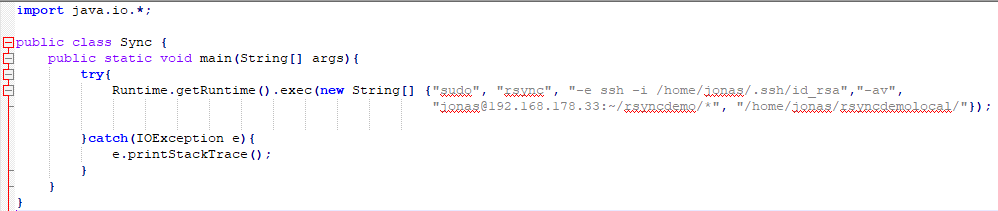
\includegraphics[width=1.0\textwidth]{JavaPrototype.png}
\\\\
Ich testete das Java-Programm zwischen meinen VMs was erfolgreich funktionierte. Ich änderte es jedoch aufgrund der oben gennanten Gründe in das unten gezeigte Bash-Skript ab. Ich synchronisierte anfangs zum Test nur einzelne Ordner und kein Dateisystem.
\\\\
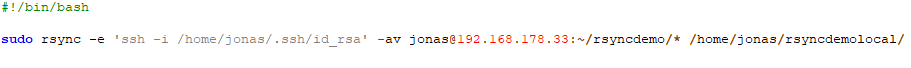
\includegraphics[width=1.0\textwidth]{syncmasterv1.png}
\\\\
Alexander passte das Bash-Skript dann so an, dass es im Labor laufen würde. Schließlich sollte es in der Lage sein mit dem Dateisystem vom Server das eigene, lokale zu Überschreiben.
Nach dem Test, bei welchem das Betriebssystem gelöscht wurde, wollte ich den Befehl am selben Tag noch fertigstellen. Diesesmal machte ich den Volltest mit kopieren und überschreiben des lokalen Dateisystems.
Der Befehl konnte noch nicht zwischen dem Pi und dem Server getestet werden, ist allerdings soweit es die VMs angeht funktionstüchtig:
\\\\
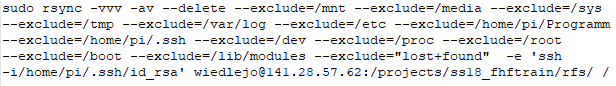
\includegraphics[width=1.0\textwidth]{skriptv3.png}
\\\\
\begin{itemize}  
\item Wir benutzen \textbf{sudo} damit der Befehl ohne Probleme ausgeführt werden kann. Da der Befehl viele Dateien überschreibt und auch löscht ist dieser Parameter vonnöten.
\item Danach wird \textbf{rsync} selbst aufgerufen
\item Die Option \textbf{-v}, gibt den Ablauf des Programms auf der Konsole aus. Da wir allerdings Fehler, die auftauchen könnten genau Untersuchen möchten, benutzen wir die Option \textbf{-vvv}, für maximale Ausgabe.
\item \textbf{Beschreibung muss noch fertig werden}
\end{itemize}

Rsync-Beschreibung  muss noch zur finalen 

Die erste Version des Services, den ich zuhause erstellte sah folgendermaßen aus:
\\\\
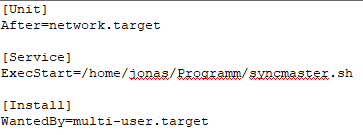
\includegraphics[width=1.0\textwidth]{servicev1.png}
Damit dieser auch an der Hochschule funktionierte musste ich allerdings ein paar Dinge ändern:
\\\\
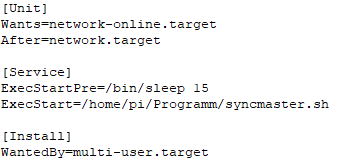
\includegraphics[width=1.0\textwidth]{servicev2.png}

Aufbau des Service:
\begin{itemize}  
\item Mit \textbf{Wants}-und \textbf{After=network-online.target} lege ich fest, dass der Service erst starten soll, wenn der Pi ein bestehende Netzwerkverbindung hat.
\item Da der Service zum Teil dennoch zu früh gestartet hat, benutze ich \textbf{ExecStartPre=/bin/sleep/ 15}, was den Service erst starten lässt nachdem 15 Sekunden abgelaufen sind.
\item \textbf{ExecStart=/home/pi/Programm/syncmaster.sh} startet dann das eigentliche Skript indem es im Programm Ordner aufgerufen wird.
\item Der Abschnitt \textbf{[Install]} legt fest wann der Service oder die Unit gestartet wird. 
\item Der Befehl \textbf{WantedBy=multi-user.target} legt fest, dass der Service startet, sobald das System hochfährt oder neugestartet wird.
\end{itemize}

fstab-Beschreibung:
\begin{itemize}
\item \textbf{fstab screenshot + aufbau}
\end{itemize}
\end{document}